% sampsize-figure4-2.tex
% The only difference between this file and sampsize-figure4.tex
% is the omission of the neuromation studies because I don't know where they go

% from http://www.texample.net/tikz/examples/consort-flowchart/
% A CONSORT-style flowchart of a randomized controlled trial
% using the PGF/TikZ package
% Author  : Morten Vejs Willert (July 2010)
% License : Creative Commons attribution license
\documentclass{article}
\usepackage[latin1]{inputenc}
\usepackage{tikz}
%%%<
\usepackage{verbatim}
%\usepackage[active,tightpage]{preview}
%\PreviewEnvironment{center}
%\setlength\PreviewBorder{10pt}%
%%%>
\begin{comment}
:Title: A CONSORT-style flowchart of a randomized controlled trial
:Tags: Matrices, Charts
:Author: Morten Vejs Willert
:Slug: consort-flowchart

A flowchart is an efficient graphical tool for depicting the 
progress of subjects through the phases of a clinical trial. 
This example shows how to use the PGF/TikZ package within a 
LaTeX article class document to make a flowchart of participants
progress through the phases of a randomized controlled trial. 
The flowchart is meant to conform to the specifications of the 
CONSORT 2010 Statement guidelines adhered to by the majority 
of scientific biomedical journals. The author takes no 
responsibility whether this goal has been achieved successfully,
should anyone care to use the example as a template when 
submitting a manuscript of their own to a biomedical journal. 

The basic code regarding placement of the nodes within a matrix, 
as well as for drawing paths between nodes, was adapted from the 
example by Kjell Magne Fauske in 'The TikZ and PGF Packages Manual 
for version 2.00' by Till Tantau.

In the example the tikzpicture-environment is used within a center
environment and \captionof from the caption package, because floating
is not required and conflicts with the preview package. In a common
document, a standard figure environment is recommended, which allows
the addition of a caption to  accompany the flowchart, as well as
options for placement of the float when typesetting the document.
\end{comment}

\usetikzlibrary{shapes,arrows}
\usepackage{caption}
\newcommand*{\h}{\hspace{5pt}}% for indentation
\newcommand*{\hh}{\h\h}% double indentation

\begin{document}
\begin{center}
  \captionof{figure}{Flowchart of participants' progress through
    the phases of the study}
  % setting the typeface to sans serif and the font size to small
  % the scope local to the environment
  \sffamily
  \footnotesize
  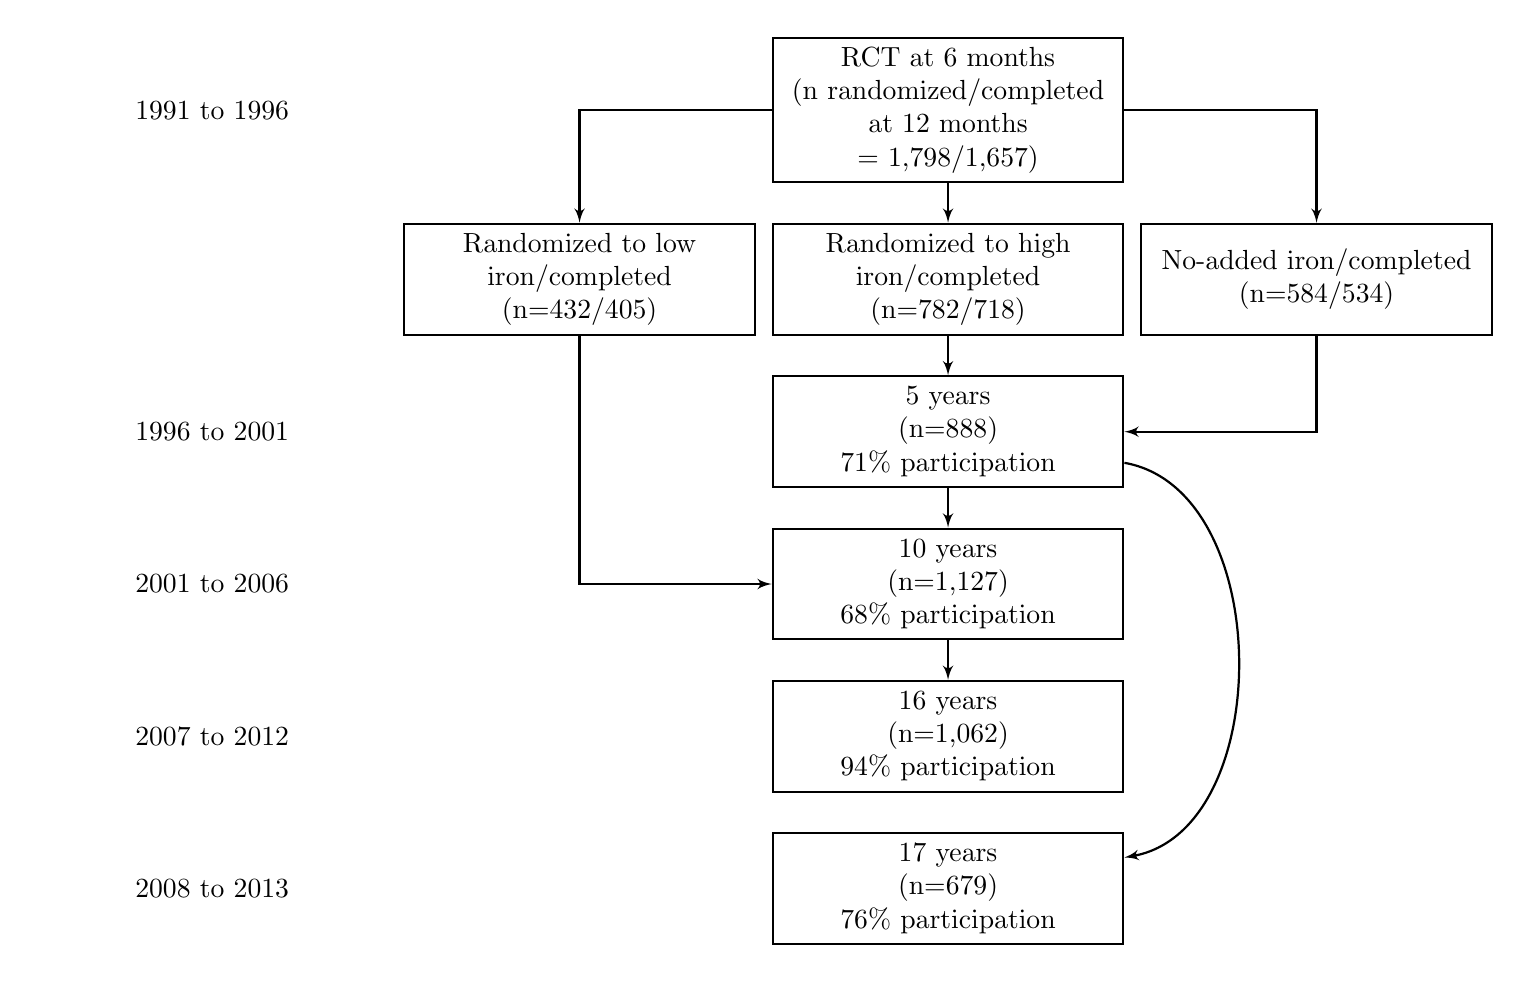
\begin{tikzpicture}[auto,
    %decision/.style={diamond, draw=black, thick, fill=white,
    %text width=8em, text badly centered,
    %inner sep=1pt, font=\sffamily\small},
    block_center/.style ={rectangle, draw=black, thick, fill=white,
      text width=12em, text centered, minimum height=4em},
    block_center2/.style ={rectangle, draw=black, thick, fill=white,
      text centered, minimum height=4em},			
    block_clear/.style ={rectangle, draw=none, thick, fill=white,
      text width=12em, text centered, minimum height=4em},
    block_left/.style ={rectangle, draw=black, thick, fill=white,
      text width=16em, text ragged, minimum height=4em, inner sep=6pt},
    block_noborder/.style ={rectangle, draw=none, thick, fill=none,
      text width=18em, text centered, minimum height=1em},
    block_assign/.style ={rectangle, draw=black, thick, fill=white,
      text width=18em, text ragged, minimum height=3em, inner sep=6pt},
    block_lost/.style ={rectangle, draw=black, thick, fill=white,
      text width=16em, text ragged, minimum height=3em, inner sep=6pt},
      line/.style ={draw, thick, -latex', shorten >=0pt}]
    % outlining the flowchart using the PGF/TikZ matrix funtion
    \matrix [column sep=2mm, row sep=5mm] {
      % start of study - row 1
      \node [block_clear] (time1) {1991 to 1996}; % watch out, dashes are special characters
			& ;
			& \node [block_center] (RCT) {RCT at 6 months\\(n randomized/completed at 12 months = 1,798/1,657)}; % got this number from Lozoff 2003 paper
			& ; \\
%      & \\;.
			\node [block_clear] (time2) {}; 
			& \node [block_center] (rand1) {Randomized to low iron/completed\\(n=432/405)}; 
			& \node [block_center] (rand2) {Randomized to high iron/completed\\(n=782/718)};
			& \node [block_center] (rand3) {No-added iron/completed\\(n=584/534)}; \\
%			& \node [block_clear] (mat0) {}; \\
			\node [block_clear] (time3) {1996 to 2001};
			& ;
			& \node [block_center] (samp5) {5 years\\(n=888)\\71\% participation};
			& ; \\
%			& ; \\
			\node [block_clear] (time4) {2001 to 2006};
			& ;
			& \node [block_center] (samp10) {10 years\\(n=1,127)\\68\% participation};
			& ; \\
%			& ; \\
			\node [block_clear] (time5) {2007 to 2012};
			& ;
			& \node [block_center] (samp16) {16 years\\(n=1,062)\\94\% participation}; % from NHLBI-WGS_RFI_v4.pdf document
			& ; \\
%			& ; \\
			\node [block_clear] (time6) {2008 to 2013};
			& ;
			& \node [block_center] (samp17) {17 years\\(n=679)\\76\% participation}; % from NHLBI-WGS_RFI_v4.pdf document
			& ; \\
%			& ; \\
    };% end matrix
    % connecting nodes with paths
    \begin{scope}[every path/.style=line]
      % paths for randomization rows
      \path (RCT)  -| (rand1);
      \path (RCT)  -- (rand2);
			\path (RCT) -| (rand3);
			% paths from infant studies to 5 year old group
			\path (rand2) -- (samp5);
			\path (rand3) |- (samp5);
			% paths from 5 year old group to 10 year old group
			\path (samp5) -- (samp10);
			\path (rand1) |- (samp10);
			% paths to 16 year old group
			\path (samp10) --  (samp16);
			% paths to 17 year old group
			\path (samp5) edge [bend left=80]  (samp17);
    \end{scope}
  \end{tikzpicture}
\end{center}
\end{document}
